%%%%%%%%%%%%%%%%%%%%%%%%%%%%%%%%%%%%%%%%%
% Beamer Presentation
% LaTeX Template
% Version 1.0 (10/11/12)
%
% This template has been downloaded from:
% http://www.LaTeXTemplates.com
%
% License:
% CC BY-NC-SA 3.0 (http://creativecommons.org/licenses/by-nc-sa/3.0/)
%
%%%%%%%%%%%%%%%%%%%%%%%%%%%%%%%%%%%%%%%%%

%----------------------------------------------------------------------------------------
%	PACKAGES AND THEMES
%----------------------------------------------------------------------------------------

\documentclass{beamer}

%\mode<presentation> {
\usetheme{Madrid}

%\setbeamertemplate{footline} % To remove the footer line in all slides uncomment this line
%\setbeamertemplate{footline}[page number] % To replace the footer line in all slides with a simple slide count uncomment this line
%\setbeamertemplate{navigation symbols}{} % To remove the navigation symbols from the bottom of all slides uncomment this line
%}

\usepackage{graphicx} % Allows including images
\usepackage{booktabs} % Allows the use of \toprule, \midrule and \bottomrule in tables

%----------------------------------------------------------------------------------------
%	TITLE PAGE
%----------------------------------------------------------------------------------------

\title[Hubness]{Project 5: The Hubness Phenomenon in High Dimensional Spaces} % The short title appears at the bottom of every slide, the full title is only on the title page

\author{} % Your name
\date{\today} % Date, can be changed to a custom date

\begin{document}

\begin{frame}
\titlepage % Print the title page as the first slide
\end{frame}

%\begin{frame}
%\frametitle{Overview} % Table of contents slide, comment this block out to remove it
%\tableofcontents % Throughout your presentation, if you choose to use \section{} and \subsection{} commands, these will automatically be printed on this slide as an overview of your presentation
%\end{frame}

%----------------------------------------------------------------------------------------
%	PRESENTATION SLIDES
%----------------------------------------------------------------------------------------

%------------------------------------------------
%\section{First Section} % Sections can be created in order to organize your presentation into discrete blocks, all sections and subsections are automatically printed in the table of contents as an overview of the talk
%------------------------------------------------

%\subsection{Subsection Example} % A subsection can be created just before a set of slides with a common theme to further break down your presentation into chunks


\begin{frame}
\frametitle{Project 5 Participants}

\begin{itemize}
\item Carlotta Domeniconi (George Mason University)
\item Sibel Tari (Middle East Technical University)
\end{itemize}

\begin{itemize}
\item G\"{u}lce Bal (Middle East Technical University)
\item Libby Beer (Institute for Defense Analyses)
\item Hillary Fairbanks (University of Colorado Boulder)
\item Priya Mani (George Mason University)
\item Jesse Metcalf-Burton (Department of Defense)
\item Marilyn Vazquez (George Mason University)
\end{itemize}
\end{frame}


\begin{frame}
\frametitle{Group 5 Overview}

\begin{itemize}
\item Overview of concepts and datasets
\item Question 1: Intrinsic dimensionality via hubness
\begin{itemize}
\item{Skewness vs. feature ranking - what is the right way to rank features?}
\item{Supervised vs. unsupervised methods} 
\end{itemize}
\item Question 2: Hubs, density, clustering, and outliers
\begin{itemize}
\item How does hubness relate to data density?
\item How are hubs distributed across clusters?
\item How do hubs relate to special points from various clustering methods (DBSCAN core points, outliers, etc.)?
\end{itemize}
\end{itemize}

\end{frame}


\begin{frame}
\frametitle{Hubness - how many nodes have me as a near neighbor?}

\centering
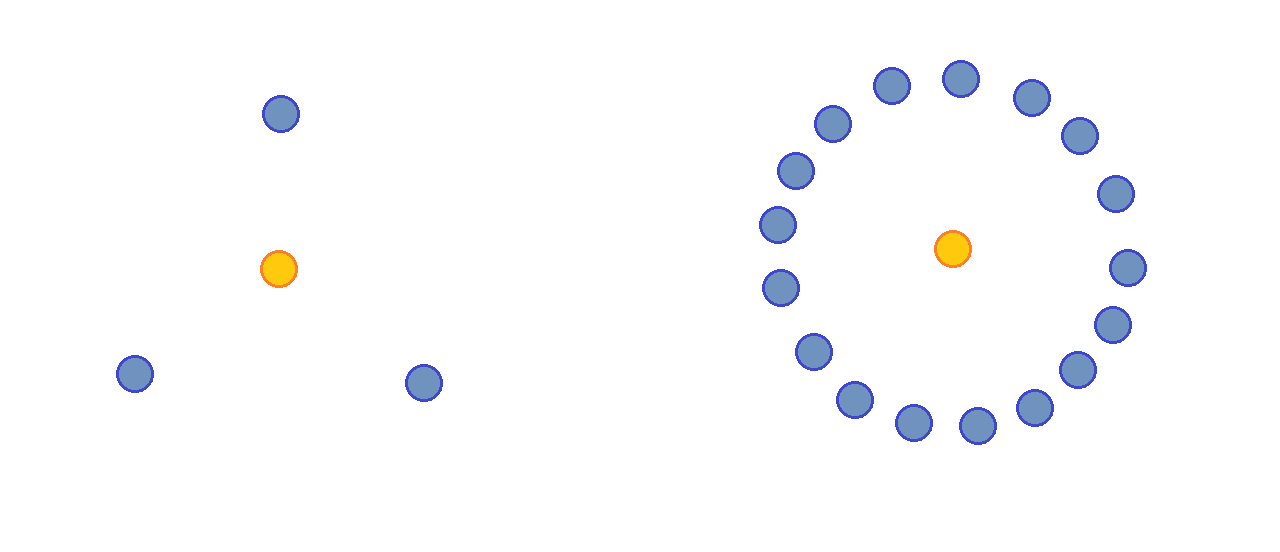
\includegraphics[width=5in]{./fig/hubness_def_1.png}

\end{frame}

\begin{frame}
\frametitle{Hubness - how many nodes have me as a near neighbor?}

\centering
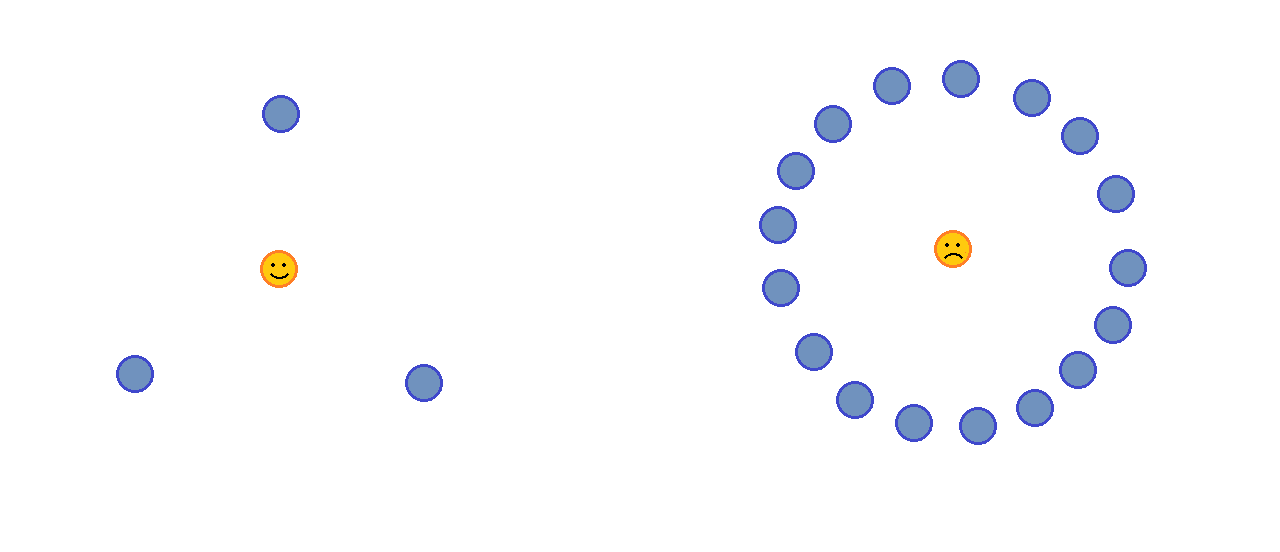
\includegraphics[width=5in]{./fig/hubness_def_2.png}

\end{frame}


\begin{frame}
\frametitle{Synthetic data -- density difference}
\centering
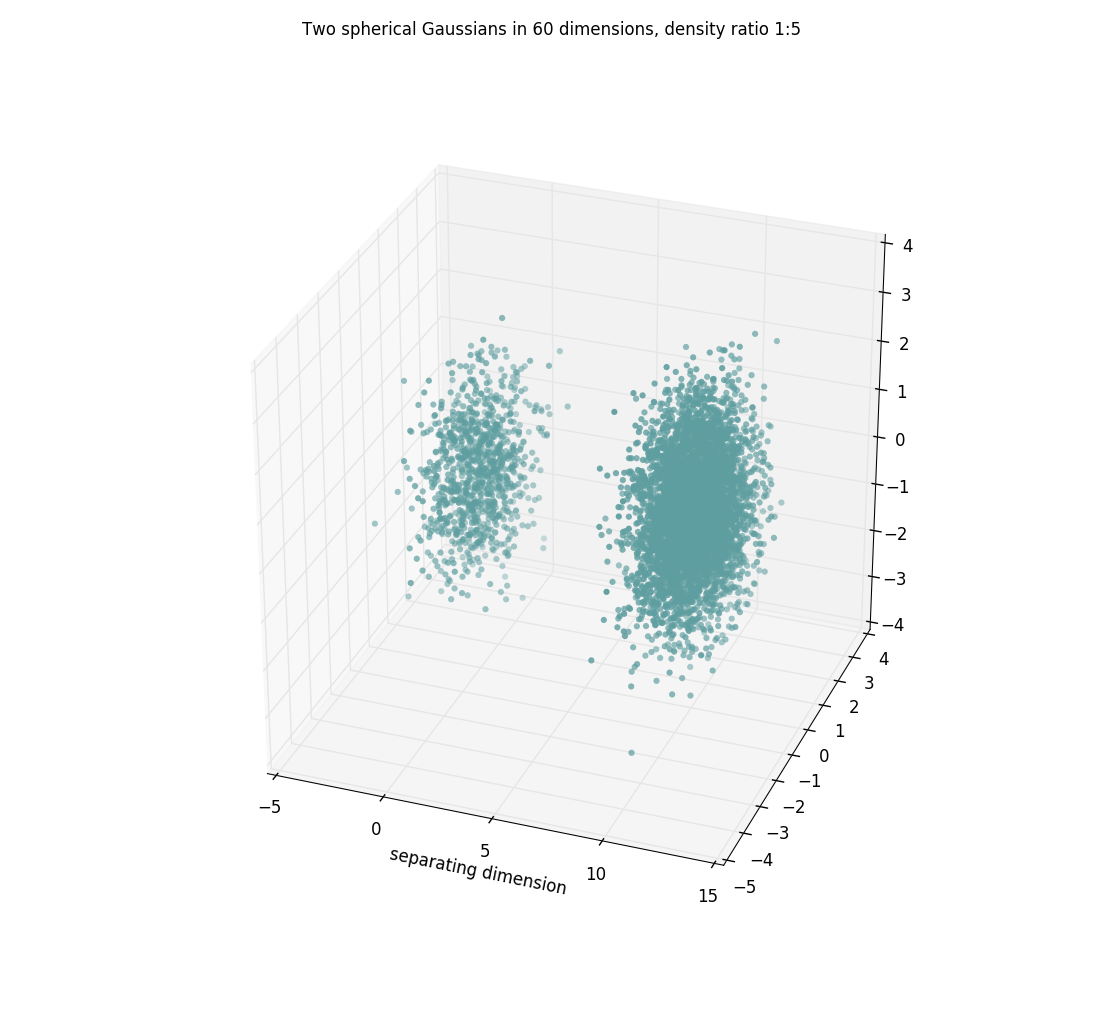
\includegraphics[height=3in]{./fig/gaussian_illustration.png}
\end{frame}

\begin{frame}
\frametitle{Synthetic data -- dimensionality difference}
\centering
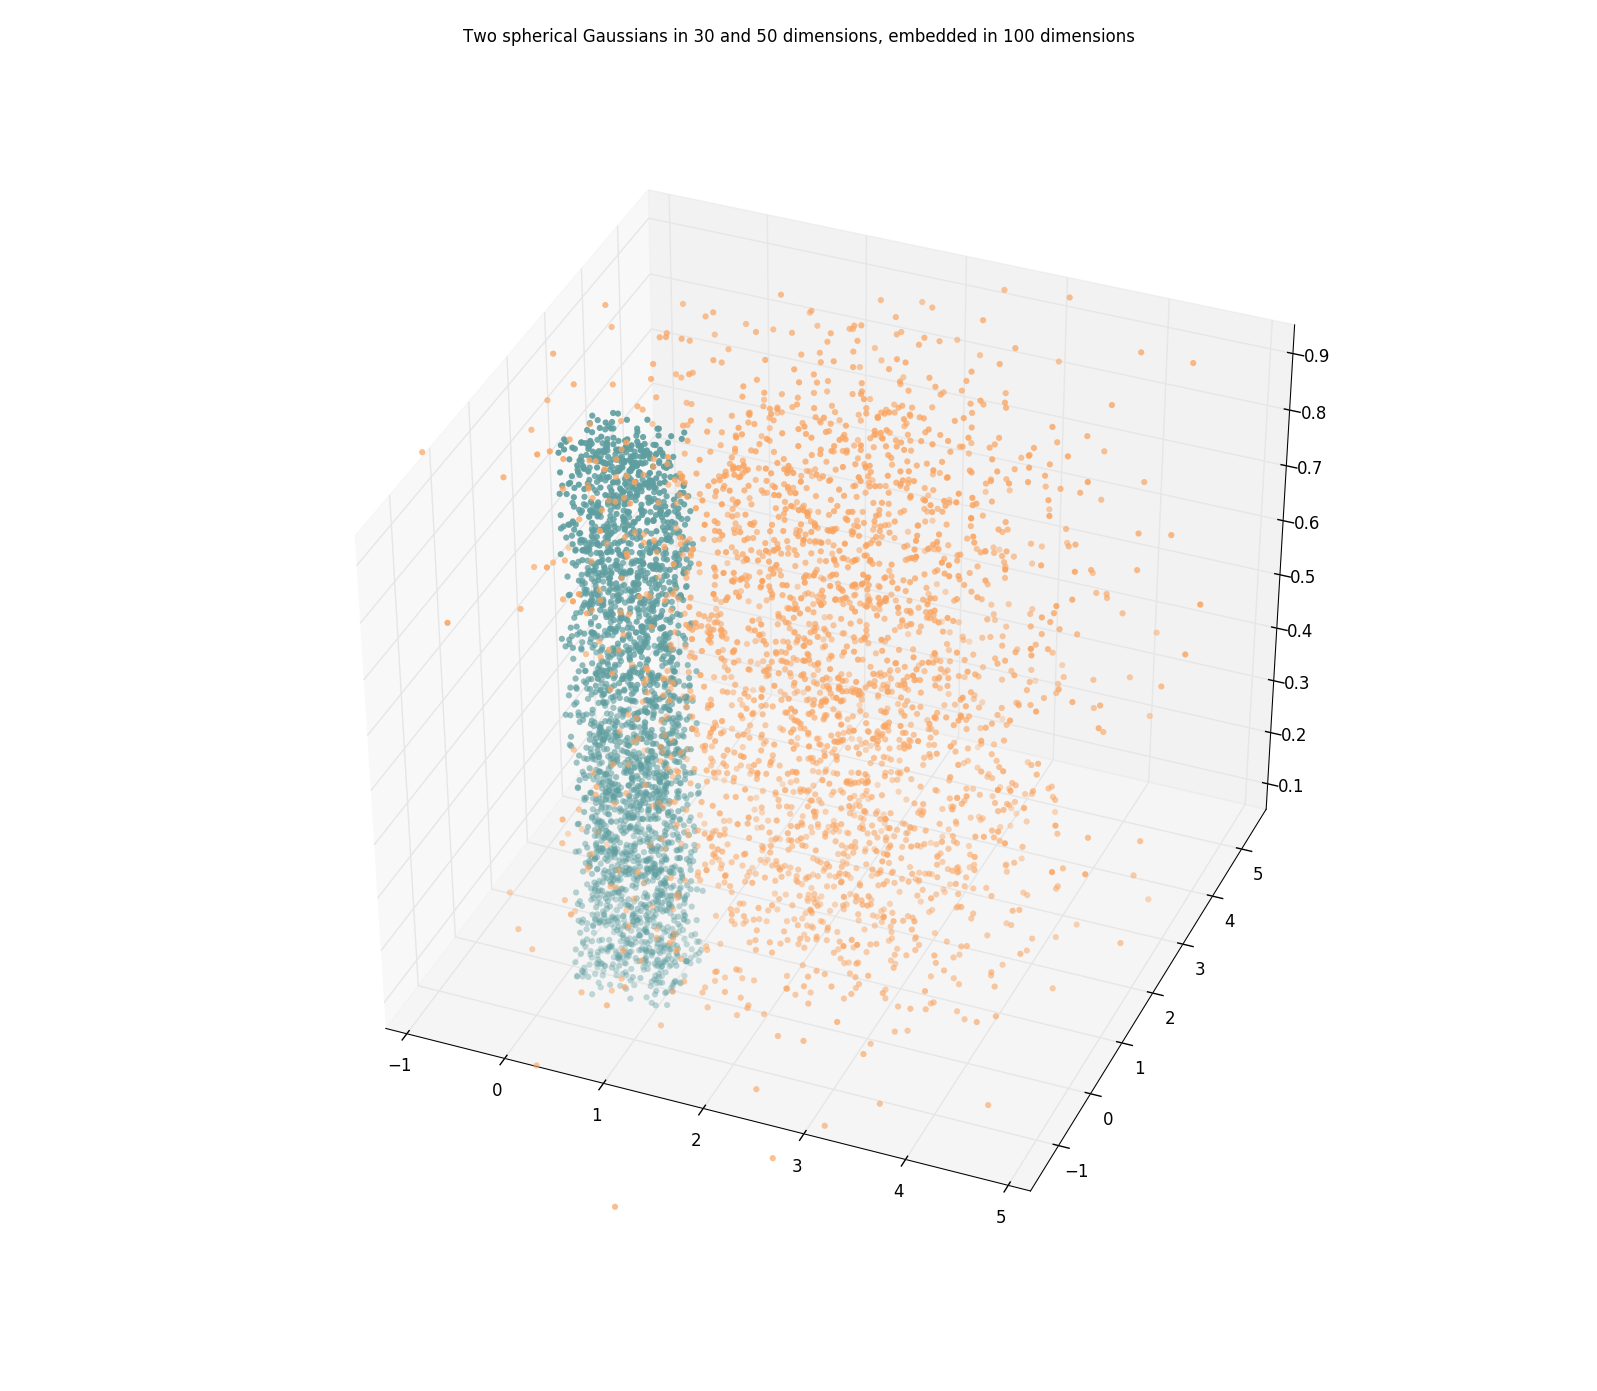
\includegraphics[height=3in]{./fig/priya_illustration.png}
\end{frame}

\begin{frame}
\frametitle{Real-world data: spam classification}
\centering
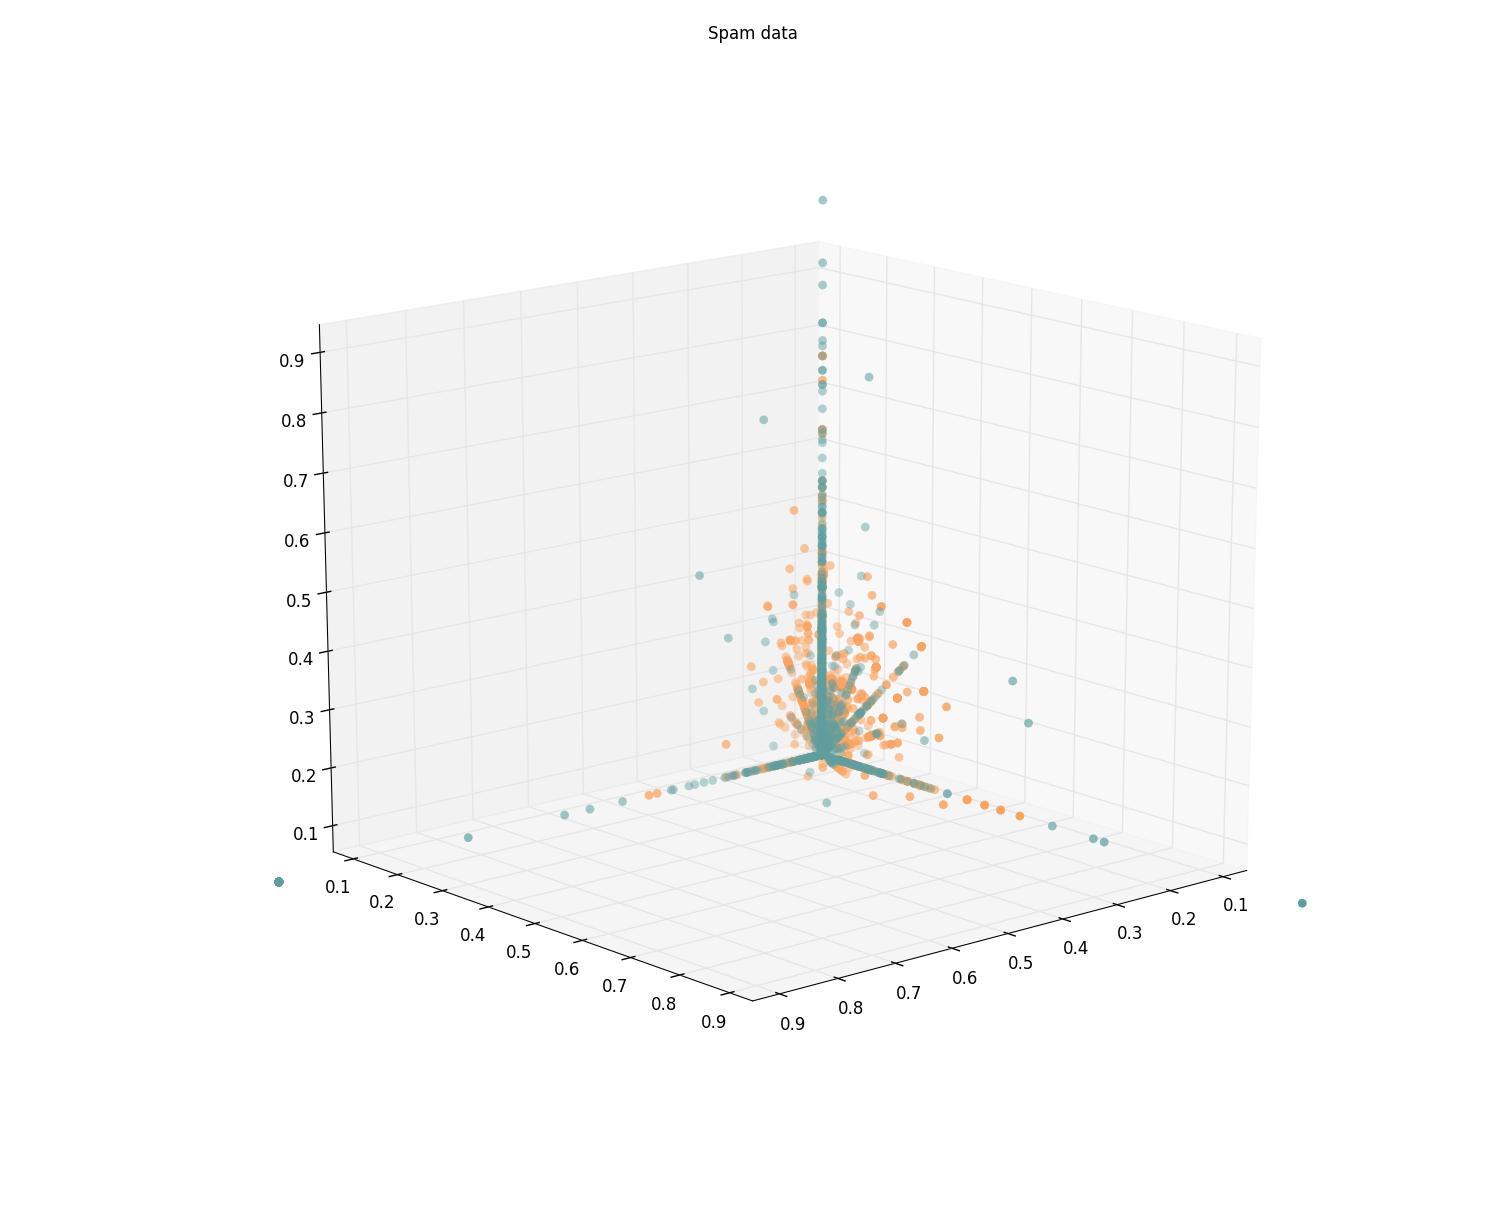
\includegraphics[height=3in]{./fig/spam_illustration.png}
\end{frame}

\end{document}
